\section{}
Consider the following system consisting of two carts connected by a damper:
\begin{figure}[h]
    \centering
    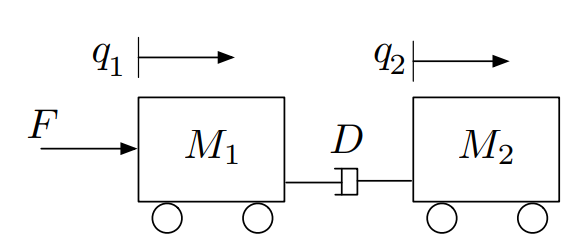
\includegraphics[width=0.5\textwidth]{Questions/Figures/Q2ProblemDiagram.png}
    \caption{System consisting of two carts connected by a damper.}
    \label{fig:Q2 System}
\end{figure}

The input is the force $F$ applied to the first cart, while $q_1$ and $q_2$ are the positions of the first and second cart, 
respectively. The output is the position of the second cart $q_2$.

\subsection{}
\textit{Using Newton’s Second Law, obtain the equations of motion of the system.}

% Figure to be included later

Since both carts are moving, the damper is applying a force based on the relative velocity of the two carts. The equation of motion for the first cart is:

\begin{equation}
    M_1\ddot{q_1} = F - D(\dot{q_2} - \dot{q_1}) \nonumber
\end{equation}

By Newton's Third Law, the damping force on the second cart is equal and opposite to the damping force on the first cart. The equation of motion for the second cart is:

\begin{equation}
    M_2\ddot{q_2} = D(\dot{q_2} - \dot{q_1}) \nonumber
\end{equation}

\subsection{}
%\textit{Introduce the state variables x1 = q1, x2 = q2, x3 = ˙q1, x4 = ˙q2. Obtain the state model of this system.}
% use math mode for the problem statement
\textit{Introduce the state variables $x_1 = q_1$, $x_2 = q_2$, $x_3 = \dot{q_1}$, $x_4 = \dot{q_2}$. Obtain the state model of this system.}

In addition to the above state variables, let the system input be $u = F$. The state model of this system is:

\begin{align*}
    \dot{x_1} &= x_3 \\
    \dot{x_2} &= x_4 \\
    \dot{x_3} &= \frac{1}{M_1}u - \frac{D}{M_1}(x_4 - x_3) \\
    \dot{x_4} &= \frac{D}{M_2}(x_4 - x_3) \\
    y &= x_2
\end{align*}

\subsection{}
\textit{Obtain the state-space form of this system.}

By inspection, the state dynamics are linear, and the output is linear. Rewriting the state model in matrix form:
\begin{align*}
    x &=
    \begin{bmatrix}
        \dot{x_1} \\
        \dot{x_2} \\
        \dot{x_3} \\
        \dot{x_4}
    \end{bmatrix}
    =
    \begin{bmatrix}
        0 & 0 & 1 & 0 \\
        0 & 0 & 0 & 1 \\
        0 & 0 & -\frac{D}{M_1} & \frac{D}{M_1} \\
        0 & 0 & \frac{D}{M_2} & -\frac{D}{M_2}
    \end{bmatrix}
    \begin{bmatrix}
        x_1 \\
        x_2 \\
        x_3 \\
        x_4
    \end{bmatrix}
    +
    \begin{bmatrix}
        0 \\
        0 \\
        \frac{1}{M_1} \\
        0
    \end{bmatrix}
    \begin{bmatrix}
        u \\
    \end{bmatrix} \\
    y &=
    \begin{bmatrix}
        0 & 1 & 0 & 0
    \end{bmatrix}
    \begin{bmatrix}
        x_1 \\
        x_2 \\
        x_3 \\
        x_4
    \end{bmatrix}
    +
    \begin{bmatrix}
        0
    \end{bmatrix}
    \begin{bmatrix}
        u \\
    \end{bmatrix}
\end{align*}